Giving importance and variety of protein-protein interactions in a cell, numerous methods were developed to discover the fact that 
two or more proteins form a complex by measuring kinetics and free energy of its formation or even by solving the atomic structure of the complex.
The openness of the proteomics community also resulted in the construction of many databases of protein-protein interactions. All experimental methods of 
identification and characterization of protein-protein interactions
can be classified using two parameters: scale(high-throuput, individual) and system( \emph{in vivo}, \emph{in vitro}). Usually, a low-throuput approach
gives much more information about interaction properties, whereas a high-throuput one only identifies the presense or absense of an interaction.

\subsection{Yeast two-hybrid method (Y2H)}
The Y2H is probably the oldest and most widespread method to identify interaction of proteins \emph{in vivo}, which was scaled up to proteome level.
In the pioneering work by Fields S. and Song  O. \cite{fields1989novel} it was shown that if the domain of the transcription activator that directs 
binding to a promoter (BD) is separated from a domain that activates transcription from this promoter (AD), the transcription is deactivated.
Based on this principle, two proteins of interest are fused to BD and AD, respectively, and the transcription of the reporter gene signals if they interact (Fig \ref{Fig:Y2H}).

\begin{figure}[H]
    \begin{centering}
      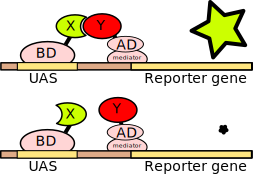
\includegraphics[width=0.5\linewidth]{Intro/Fig/Y2H.pdf}  
      \caption[Y2H explanation]{Schematic representation of the Y2H method. If the two protein X and Y do interact, expression of the reporter gene is high (yellow star), otherwise
      AD and BD domains of the promoter are separated and the expression is low. UAS stands for the upstream regulating sequence.}
      \label{Fig:Y2H}
    \end{centering}
\end{figure}

The are at least two scaling schemes: matrix and library approaches \cite{uetz2000comprehensive,ito2001comprehensive}. In the first one, 
clones expressing different proteins ${X_i}$ are taken and plated each
in the rows of wells on a plate. The same set of clones is plated in colums of wells on a plate. Then, when the two yeast cells in each well mate and make a diploid that
expresses both proteins $X_i$ and $X_j$. Afterwards, the expression of a reporter gene in a cell $i,j$ means that proteins $X_i$ and $X_j$ interact.
In the library-based approach, clones containig protein $X_i$ are screened agains a library of clones with various proteins, which can be expressed from
random cDNA or all open reading frames of a certain genome. In this case, the diploids expressing interacting proteins are selected agains specific growing media.
The proteins that interact with $X_i$ are determined by the DNA sequencing.

\subsection{Mass spectrometry and tandem affinity purification}
In this method, a certain protein is fused with the DNA sequence that expresses the TAP tag (IgG binding domains of \emph{Staphylococcus} protein A and calmodulin
binding peptide separated by the TEV protease site \cite{puig2001tandem}). When the DNA construct is expressed in a host, it produces the protein of interest that forms complexes
with other proteins of the host. During the purification, these protein complexes bind to the IgG matrix. Other proteins that did not form complexes with
the TAP-tagged one, hop through the matrix. Afterwards, using TEV protease, one cleaves of IgG binding domains and purified complexes are eluated from the matrix.
The second purification step is the binding to calmodulin-coated beads. The simple representation of the two-step purification is shown on Fig. \ref{Fig:TAP}.
Finally, the eluate is loaded to the SDS-PAGE gel and the resulting bands are cleaved by proteases.

After the purification, one uses mass-spectrometry to identify the fragments of the cleaved protein-protein complexes \cite{di2005molecular}. Mass-spectrometry identifies particles 
based on their charge-to-mass ration. It allows to recognize fingerprints of short peptides and therefore identify the proteins using the solution of 
peptide fragments.
A certain advantage of the TAP-MS method over Y2H is that it can detect not only dimeric protein-protein interaction, but also multimeric complexes.

\begin{figure}[H]
    \begin{centering}
      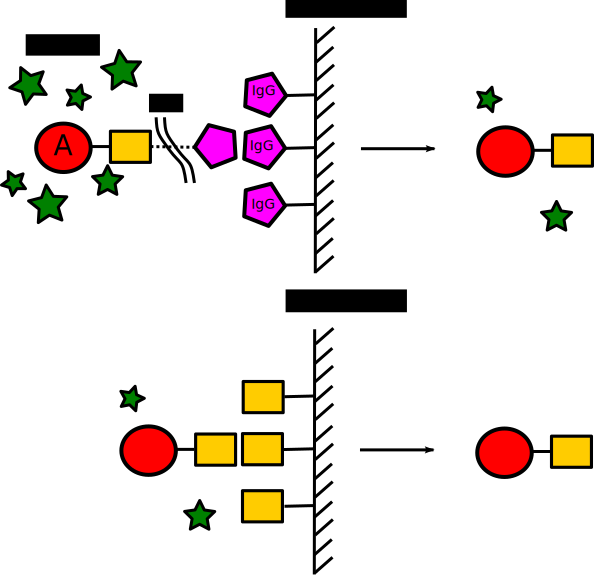
\includegraphics[width=0.5\linewidth]{Intro/Fig/TAP.pdf}  
      \caption[TAP-MS explanation]{Schematic representation of the tandem affinity pyrification method. Contaminants are shown with green stars, IgG binding domain is shown with 
      pink pentagon (as well as the IgG coating) and calmodulin (as well as calmodulin coating) is shown with squares.}
      \label{Fig:TAP}
    \end{centering}
\end{figure}

\subsection{Gene co-expression}
Recently the methods that allowed measuring expression of the genes on the scale of the whole cell were invented. Using this methodology,
one can measure the similarity of expression profiles over different conditions of the two or more genes that code for interacting proteins. 
It turns out that they are significantly more similar than the gene expression profiles of random non-interacting proteins \cite{jansen2002relating}.

\subsection{Synthetic lethality}
The mutations in the genome of an organism affect its phenotype. In many cases this phenotype alternation is caused by the change in the protein-protein interaction
network. By introducing random mutations or deletions in the genes of two proteins, one can monitor survival rate of these cells. The lethality of one such mutation 
can point to presence of interaction between the two target proteins \cite{ooi2006global}.

\subsection{Fluorescence resonance energy transfer}
The fluorescence resonance energy transfer (FRET) occurs between two molecules: one (donor) in an excited state and the orther (aceptor) in the ground state. 
The energy is transfered through the dipole-dipole interaction between the molecules and does not involve emission \cite{yan2003analysis}. The probability of such transfer to occur
strongly depends on the distance between the donor and the aceptor. However, it is almost independent of the environmental conditions, which makes this method a great
tool to study molecular interactions \emph{in vivo}. More specifically, the two fluorophores are fused to the two proteins of interest (Fig. \ref{Fig:FRET}). One is then excited using 
a laser and if these molecules form a complex, it transfers energy to the second fluorophore that emits light at a certain wavelength. One of examples
of FRET application is the investigation of membrane proteins dimerization \emph{in vivo}, in particular of melatonin receptor types 1A and 1B \cite{ayoub2004preferential}.

\begin{figure}[H]
    \begin{centering}
      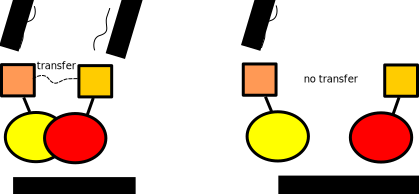
\includegraphics[width=0.5\linewidth]{Intro/Fig/FRET.pdf}  
      \caption[FRET explanation]{Schematic representation of the fluorescence resonance energy transfer method. If the two proteins interact, the fluorophores (blocks) come close and the energy
      transfer between them becomes possible. Therefore, exciting one fluorophore, one detects the emission from another. Otherwise, if the proteins do not interact,
      no emission of the second fluorophore is detected upon excitation of the first one.}
      \label{Fig:FRET}
    \end{centering}
\end{figure}

\subsection{Isothermal titration calorimetry}
This method allows to measure stoichiometry, dissociation constant, enthalpy and entrophy of the binding reaction between two proteins \cite{velazquez2005itc}. 
The experimental setup consists of two thermally isolated chambers.
One of the chambers is used as a reference and is filled with water. The other contains one of the interacting proteins. Its interaction partner is titrated in a known amount to the chamber. 
The thermometer measures temperature difference between these
two chambers and controls heaters to equilibrate their temperature (while maintaining the temperature of the reference chamber constant). 
The amount of heat spent to make the two chamber isothermic is measured during the experiment. 
Figure \ref{Fig:ITC} shows a schematic example of data obtained from an ITC experiment. The red line shows the peaks of energy transfer that correspond to titration events. Fitting 
these peaks with the interaction model (blue dashed line on Fig. \ref{Fig:ITC}) of a titration substance and a substance in the reservoir one can deduce the parameters of the model. 
In the simplest case of protein-ligand interaction one obtains enthalpy, dissociation constant and stoichiometry of the reaction.

\begin{figure}[H]
    \begin{centering}
      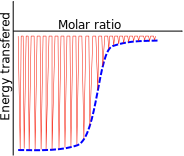
\includegraphics[width=0.5\linewidth]{Intro/Fig/ITC.pdf}  
      \caption[Isothermal titration calorimetry explanation]{Schematic representation of the data obtained from an isothermal titration calorimetry device. The red line 
      shows the energy transfered from the reservoir with the protein to the reference reservoir. Blue dashed line is an example of model fitted to the data.}
      \label{Fig:ITC}
    \end{centering}
\end{figure}

\subsection{Nuclear magnetic resonance spectroscopy (NMR)}
This method is based on the absorbtion and emission of radio-frequency radiation by the nuclei of certain atoms. The emission and absorbtion spectra depend on the 
environment of nuclei and therefore the measurement allows to reconstruct the distance matrix between certain atoms in a protein in solution. This method also
allows to measure the dynamics of proteins and their interaction. The classical approach is based on the Nuclear Overhauser Effect (NOE). One of the examples of the NMR results is
the structure of the Twist protein, a transcription factor that plays a key role in the epithelial-mesenchymal transition and the bromodomain-containing protein 4 \cite{shi2014disrupting} 
(see Fig. \ref{Fig:TwistBRD4}). Due to the complexity of spectra measured during the experiment, this approach is limited to protein complexes of the size up to 300 amino acids.

\begin{figure}[H]
    \begin{centering}
      \includegraphics[width=0.5\linewidth]{Intro/Fig/TwistBRD4.png}  
      \caption[The structure of Twist protein with the Brd4 protein]{The structure of Twist protein(green) with the bromodomain-containing protein 4 (red) measured using NOE-NMR technique \cite{shi2014disrupting}.
      PDB code 2MJV.}
      \label{Fig:TwistBRD4}
    \end{centering}
\end{figure}

\subsection{Cryo electron microscopy}
The broad variety of methods go under the name of Cryo electron microscopy (Cryo-EM). The basic principle underlying this method is the same as in the conventional
light microscopy. The difference lies in the radiation source. In Cryo-EM, the electron beam accelerated up to 300kV is used. This allows increasing the resolution that 
depends on the wavelength of the incident radiation, up to atomic one (wavelength of electrons accelerated by 300kV is about $0.02$\AA). However, the increased resolution
goes with the increased radiation dammage to the sample. Variety of methods are used to diminish ionizing effect of electrons on the biological samples. More precisely, 
measurement are conducted at low temperatures \cite{dubochet1988cryo}, averaging many identical units \cite{taylor1974electron}, single-particle microscopy.
The last one is probably the most used one in structural biology. 

The single-particle Cryo-EM is based on collecting information from many 2D projections of an object to reconstruct its 3D low-resolution model (electron density map, EDM). 
Afterwards, the supplementary information provided by NMR of X-Ray crystallography is used to construct an atomistic model of the object.

The 3D reconstruction of the EDM is usually based on the central projection theorem. It states that the Fourier images of 2D projections of a 3D object are the central slices of
its 3D Fourier images. The relative positioning of two projections can be derived from the common lines in their Fourier images. These algorithms
are implemented in the programs like IMAGIC \cite{van1996new}, SPIDER \cite{shaikh2008spider}, FREALIGN \cite{grigorieff2007frealign} \emph{etc}.

The resolution that can be obtained using this technique is highly dependent on the symmetry of the object measured. For example, highly symmetric icosahedral viruses 
envelopes were measured with up to 3\AA~ resolution \cite{zhang20103}. The other examples of reconstructed protein complexes usually have resolution in the range of 7\AA - 15\AA.
This method is the main source of information on the large protein-protein assemblies today, like ribosomes \cite{penczek2011identifying} and chperonines \cite{cong20104}.

\subsection{X-ray crystallography}
The X-ray crystallography is the most time- and cost- demanding method, but it provides the most detailed atomistic information on the structure of protein-protein 
complexes. The starting point of this technique is a protein crystal. Obtaining crystal of a certain protein-protein complex is often the major hurdle 
and sometimes even impossible. Large protein-protein complexes and membrane proteins are especially hard to crystallize. Nontheless, the X-ray crystallography 
remains a major method to study structures of protein-protein complexes. The method is based on the diffraction of X-rays on the atoms, arranged in a lattice.
The crystal of a protein is rotated with respect to the incident beam and the diffraction patterns are measured for each rotation. From these patterns
one can reconstruct the absolute values of the Fourier image of a unit cell of the crystal. Afterwards, the phases of the Fourier image have to be reconstructed
or measured. One of the most used way to obtain the phasing is the so-called molecular replacement. This means that approximate theoretical molecular structure of
the unit cell is fitted into the given dataset. Afterwards, one minimizes discrepancy of the fitted structure with the diffraction pattern and obtains the final one.
The quality of the final structure is judged by the R-factor. It shows to what extent the resulting structure explains the diffraction peaks.
